\section{Rete neurale}
\label{Rete neurale}

La libreria utilizzata per sviluppare la Rete neurale \`e stata \textit{ConvNetJS}. L'aspetto positivo di tale scelta \`e stata la semplicit\`a nell'utilizzo del linguaggio javascript; l'aspetto negativo ha riguardato la totale mancanza di mantenibilit\`a della libreria stessa che comporta la scarsit\`a di esempi applicativi, oltre alla documentazione ufficiale, che costringono lo sviluppatore ad una ricerca approfondita personale in un ambiente ove lo nozioni si presentano scarse e a continue prove per verificare la validit\`a del codice prodotto.
\begin{figure}[H]
\centering
	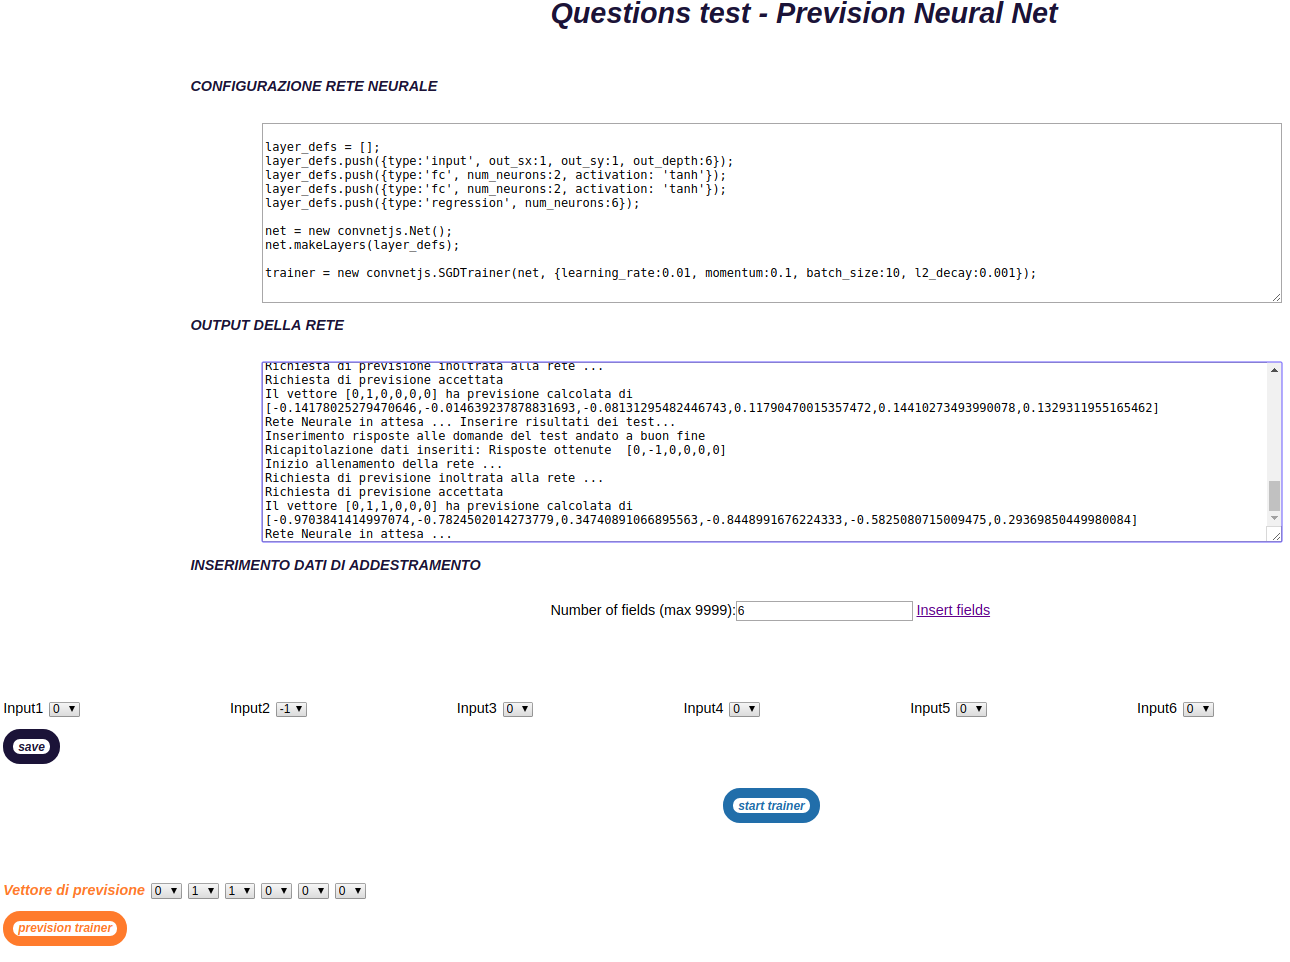
\includegraphics[width=1\linewidth]{./image/GUI-rete-neurale.png}
	\caption{Interfaccia utente della Rete neurale di prova.}
\end{figure}
\noindent
Durante il periodo 24/05 - 31/05 mi sono occupata dello sviluppo di una Rete neurale in grado di ricevere in input un training set di dimensione 6 e di restituire una previsione sui dati di apprendimento ricevuti.
\noindent
Il problema che la rete mira ad analizzare \`e quello discusso nel precedente capitolo \textit{Analisi dei dati di probabilit\`a}
\\\\
Per agevolare l'apprendimento della rete, ed ottenere delle previsioni stabili mi sono occupata di implementare due metodi di generazione randomica di dati in modo da far apprendere massicciamente la stessa.
Il dato prodotto consiste in un vettore di 6 elementi, composto da  -1, 0 e 1 con il seguente criterio:
\begin{itemize}
\item \textbf{-1}: la domanda x \`e stata posta al candidato che ha risposto in maniera errata;
\item \textbf{0}: la domanda x non \`e stata posta al candidato;
\item \textbf{1}: la domanda x \`e stata posta al candidato che ha saputo rispondere correttamente.
\end{itemize}
\noindent
Il primo metodo che ho sviluppato si occupa di generare un vettore di dati di apprendimento basandosi esclusivamente su come le domande sono interconnesse tra di loro (grazie all'uso di un grafo della conoscenza costruito ad hoc); il secondo metodo ripropone quanto perseguito dal primo metodo con il valore aggiunto di generazione di un profilo randomico di un candidato, che tiene conto della  probabilit\`a di risposta ad una domande seguendo la formula P(A)= $\frac{1}{3}+\frac{1}{6}P(S_1)+\frac{2}{3}P(S_2)$.

\subsection{Test effettuati}
\label{Test effettuati}

Alcune decisioni che ho preso durante la configurazione della rete riguardano i seguenti settori:
\begin{enumerate}
\item Una rete neurale non deve, per fornire dei dati attendibili, possedere un numero di neuroni troppo elevato rispetto al trainset effettuato; altrimenti la previsione  ritornerebbe l'identit\`a del vettore di input della stessa, come conseguenza diretta della capacit\`a troppo elevata di immagazzinare dati.
\item I layers, ho deciso, di allenarli mediante tecnica di regressione, che permette l'inserimento in input di una funzione obiettivo e l'ottenimento di un risultato, in output, anche in virgola mobile e composto di tanti elementi quanti sono i neuroni di regressione dichiarati. Per la mia rete di prova \`e necessario dichiarare  6 neuroni in regressione perch\`e l'output, appunto, che ci si aspetta dal sistema \`e di 6 elementi.
\item Per costruire un dataset di dati consistente che permettesse alla rete di imparare qualcosa ho costruito un grafo della conoscenza con lo scopo di mettere in relazione degli argomenti che coinvolgono uno o pi\`u domande.
\begin{figure}[H]
\centering
	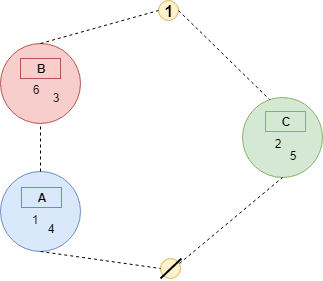
\includegraphics[width=0.60\linewidth]{./image/grafo_trainset.png}
	\caption{Grafo rappresentante le relazioni esistenti tra il set di domande di prova.}
\end{figure}
\noindent
Per svolgere l'apprendimento ogni vettore, facente parte del dataset, viene dato in pasto alla rete che a sua volta provvede alla sua assimilazione come conoscenza mediante la tecnica dell'autoencoder, ovvero la rete impara il vettore riducendone lo spazio occupato.
\item Per creare il dataset ho ritenuto sufficiente generare \textit{2000} vettori di risposta in modo da compiere in maniera esaustivo l'apprendimento della rete.
\end{enumerate}
\noindent
Il vettore passato in input per svolgere le previsioni \`e \textit{[0,0,0,0,0,0]},\textit{[0,0,1,0,1,0]} e \textit{[0,0,-1,0,0,0]}\\
Le aspettative riguardano la previsione di risposta di un candidato
\noindent. 
Di seguito riporto quanto \`e stato rilevato in fase di test.

\subsubsection{Configurazione della rete: 4 neuroni per ciascuno dei 2 layers}
\label{Configurazione della rete: 4 neuroni per ciascuno dei 2 layers}

Configurazione della rete utilizzata:\\
\begin{verbatim}layer_defs = [];
layer_defs.push({type:'input', out_sx:1, out_sy:1, out_depth:6});
layer_defs.push({type:'fc', num_neurons:4, activation: 'tanh'});
layer_defs.push({type:'fc', num_neurons:4, activation: 'tanh'});
layer_defs.push({type:'regression', num_neurons:6});

net = new convnetjs.Net();
net.makeLayers(layer_defs);

trainer = new convnetjs.SGDTrainer(net, {learning_rate:0.01,
 momentum:0.1, batch_size:10, l2_decay:0.001});
\end{verbatim}
\noindent
I layers utilizzati sono 2 e compositi da 4 neuroni.

\paragraph{Training set standard a 4 neuroni per ciascuno dei 2 layers}\mbox{}
\label{Training set standard a 4 neuroni per ciascuno dei 2 layers}
\\
\noindent
\begin{itemize}
\item \begin{verbatim}Il vettore [0,0,0,0,0,0] ha previsione calcolata di [-0.021598804903572744,-0.1372509042342871,0.06611969158456255
,0.018121335417653706,-0.11264571886853292,0.17520370837747462]\end{verbatim}
Appaiono in relazione le domande 1, 2, 5 e 3, 4, 6.\\
Gli scostamenti tra le coppie 2, 5 e 3, 6 sono consistenti con quelle che sono le relazioni di dipendenza, invece 1, 4 ha una differenza di 0.016 circa che parte da qualche millesimo fino 0.5
Le domande 3 e 6 si dovrebbero presentare con una positivit\`a inferiore rispetto a 1 e 4; nel test in analisi questo non viene rispettato da nessuna delle coppie in analisi per differenze che vanno da qualche millesimo fino a 0.018 circa.
\paragraph{Osservazioni}\mbox{}
\label{Osservazioni su rete a 4 neuroni per ciascuno dei 2 layers}
\\\\
\noindent
La configurazione testata si compone di 4 neuroni a layer su una base di 2000 test correndo il rischio di avere una rete che apprende troppo e come effetto negativo "veda" addirittura cose che non esistono. A prova di ci\`o sono i risultati non conformi alle attese.
Dunque mi fermo qui con il test di tale configurazione e riducendone il numero di neuroni presenti in ciascun layers e/o il numero di layers presenti.\\

Le nuove configurazione su cui ho effettuato i test sono esposte nei paragrafi seguenti.

\subsubsection{Configurazione della rete a 2 neuroni per ciascuno dei 2 layers}
\label{Configurazione della rete a 2 neuroni per ciascuno dei 2 layers}
Configurazione della rete utilizzata:\\
\begin{verbatim}layer_defs = [];
layer_defs.push({type:'input', out_sx:1, out_sy:1, out_depth:6});
layer_defs.push({type:'fc', num_neurons:2, activation: 'tanh'});
layer_defs.push({type:'fc', num_neurons:2, activation: 'tanh'});
layer_defs.push({type:'regression', num_neurons:6});

net = new convnetjs.Net();
net.makeLayers(layer_defs);

trainer = new convnetjs.SGDTrainer(net, {learning_rate:0.01,
 momentum:0.1, batch_size:10, l2_decay:0.001});
\end{verbatim}
\noindent
I layers utilizzati sono 2 compositi da 2 neuroni.

\paragraph{Training set standard su rete a 2 neuroni per ciascuno dei 2 layers}\mbox{}
\label{Training set standard su rete a 2 neuroni per ciascuno dei 2 layers}
\\
\noindent
\begin{itemize}
\item \begin{verbatim}[Il vettore [0,0,0,0,0,0] ha previsione calcolata di
[0.31232372051574936,0.7253754889487585,-0.5051208979797573,
0.32075742158673093,0.7324947496336937,-0.4348299972940168]
\end{verbatim}
Appaiono in relazione le domande 1, 2, 4, 5 e 3, 6.\\
Gli scostamenti tra le coppie 1, 4 e 3, 6  e 2, 5 sono consistenti con quelle che sono le relazioni di dipendenza fra le domande.
Le domande 3 e 6 si dovrebbero presentare con una positivit\`a inferiore rispetto a 1 e 4; in questo test la regola viene rispettata pienamente.\\
Dall'immagine canvas e dai dati della previsione si nota come il candidato ha una buona probabilit\`a di saper rispondere alla coppia 1 e 4, e ancora pi\`u elevata di saper rispondere correttamente alla coppia 2 e 5; molto bassa di saper rispondere correttamente alle 3 e 6 che sono, appunto, di una difficolt\`a maggiore rispetto alla coppia 1 e 4.

\item \begin{verbatim}Il vettore [0,0,1,0,1,0] ha previsione calcolata di
[0.5123144717131076,0.9123354449531641,0.2837937822420923,
0.46449868699771607,0.9029832167165894,0.3227303792035435]
\end{verbatim}
Appaiono in relazione le domande 1, 2, 3  4, 5, 6.\\
Gli scostamenti tra le coppie 1, 4 e 3, 6  e 2, 5 sono consistenti con quelle che sono le relazioni di dipendenza fra le domande.
Le domande 3 e 6 si dovrebbero presentare con una positivit\`a inferiore rispetto a 1 e 4; in questo test la regola viene rispettata pienamente.\\
Dall'immagine canvas e dai dati della previsione si nota come il candidato ha un'ottima probabilit\`a di saper rispondere alla coppia 2 e 5 (come imposto dal vettore previsione), buona di saper rispondere alla coppie 3 e 6 (come imposto dal vettore previsione) e pi\`u che buona  di saper rispondere alle 1 e 4, che sono di una semplicit\`a pi\`u elevata rispetto alla 3 e 4.
\end{itemize}

\item \begin{verbatim}Il vettore [0,0,-1,0,0,0] ha previsione calcolata di
[0.3698539826215957,0.288907514487717,-0.8504159455662308,
0.3663192502433841,0.2937448801761998,-0.7845589473185985]
\end{verbatim}
Appaiono in relazione le domande 1, 2, 4, 5 e 3, 6.\\
Gli scostamenti tra le coppie 1, 4 e 3, 6  e 2, 5 sono consistenti con quelle che sono le relazioni di dipendenza fra le domande.
Le domande 3 e 6 si dovrebbero presentare con una positivit\`a inferiore rispetto a 1 e 4; in questo test la regola viene rispettata pienamente.\\
Dall'immagine canvas e dai dati della previsione si nota come il candidato ha una discreta probabilit\`a di saper rispondere alla coppia 2 e 5, un p\`o meglio di saper rispondere alla coppie 1 e 4 e pi\`u di non saper saper rispondere alle 3 e 6 (come imposto dal vettore previsione).
\end{itemize}

\paragraph{Training set con generazione del profilo di un candidato e calcolo delle probabilit\`a di risposta a 2 neuroni per ciascuno dei 2 layers}\mbox{}
\label{Training set con generazione del profilo di un candidato e calcolo delle probabilita di risposta a 2 neuroni per ciascuno dei 2 layers}
\\
\noindent
\begin{itemize}
\item \begin{verbatim}Il vettore [0,0,0,0,0,0] ha previsione calcolata di
[0.057781303506280995,0.0513731100126314,-0.06600467867066256,
0.029940883111932555,-0.019564515397168573,-0.09570617900597932]
\end{verbatim}
Appaiono in relazione le domande 1, 2, 4 e 3, 5, 6.\\
Gli scostamenti tra la coppia 1, 4 e 3, 6 sono consistenti con  quelle che sono le relazioni di dipendenza fra le domande; invece per la coppia 2 e 5 i segni sono opposti con una differenza di 0.024.
Le domande 3 e 6 si dovrebbero presentare con una positivit\`a inferiore rispetto a 1 e 4, la regola viene rispettata pienamente. Le anomalie riscontrate sono da ricondurre alla natura del vettore di training che si basa sul calcolo della probabilit\`a di una risposta che sul grafo della conoscenza.

\item \begin{verbatim}Il vettore [0,0,1,0,1,0] ha previsione calcolata di
[0.19494624113789977,0.1712744021266377,0.577963304906936,
0.781098215373483,0.3774535909060714,0.03617314870307162]
\end{verbatim}
Appaiono in relazione le domande 1, 2, 3, 4, 5, 6.\\
Gli scostamenti tra le coppie 1 e 4 , 2 e 5, 3 e 6 sono consistenti con quelle che sono le relazioni di dipendenza fra le domande.
Le domande 3 e 6 si dovrebbero presentare con una positivit\`a inferiore rispetto a 1 e 4, la regola non viene rispettata dalla domanda 1 in rapporto con la domanda per una differenza di 0.37 circa.
Le anomalie riscontrate sono da ricondurre alla natura del vettore di training che si basa sul calcolo della probabilit\`a di una risposta che sul grafo della conoscenza.

\item \begin{verbatim}Il vettore [0,0,-1,0,0,0] ha previsione calcolata di
[0.09845785763965222,0.015421380649956663,-0.5138068038427066,
-0.4853190165287735,-0.22629262719814794,0.0008152164571250502]
\end{verbatim}
Appaiono in relazione le domande 1, 2, 6 e 3, 4, 5.\\
Gli scostamenti tra le coppie 1, 4 e 2, 5 e 3, 6 per una differenza tuttavia trascurabile  che oscilla dallo 0.2 allo 0.5.
Le domande 3 e 6 si dovrebbero presentare con una positivit\`a inferiore rispetto a 1 e 4, la regola non vale per la coppa 6 e 4.
Le anomalie riscontrate sono da ricondurre alla natura del vettore di training che si basa sul calcolo della probabilit\`a di una risposta che sul grafo della conoscenza.
\end{itemize}


\paragraph{Osservazioni}\mbox{}
\label{Osservazioni su rete a 2 neuroni per ciascuno dei 2 layers}
\\\\
\noindent
Confrontando i risultati ottenuti dalla rete con i layers impostati a 4 neuroni con quanto emerso dai dati risultanti dalla  rete a 2 neuroni emerge come la configurazione a 2 neuroni a layers \`e sicuramente quella che da i risultati attesi.\\
Quanto emerso di discordate dal secondo training set \`e come da aspettative da associare alla natura stessa della creazione del set di dati.


\subsubsection{Configurazione della rete a 4 neuroni per 1 layer}
\label{Configurazione della rete a 4 neuroni per 1 layer}

Configurazione della rete utilizzata:\\
\begin{verbatim}layer_defs = [];
layer_defs.push({type:'input', out_sx:1, out_sy:1, out_depth:6});
layer_defs.push({type:'fc', num_neurons:4, activation: 'tanh'});
layer_defs.push({type:'regression', num_neurons:6});

net = new convnetjs.Net();
net.makeLayers(layer_defs);

trainer = new convnetjs.SGDTrainer(net, {learning_rate:0.01,
 momentum:0.1, batch_size:10, l2_decay:0.001});
\end{verbatim}
\noindent
Viene utilizzato un unico layer da 4 neuroni.

\paragraph{Training set standard su rete a 4 neuroni per 1 layer}\mbox{}
\label{Training set standard su rete a 4 neuroni per 1 layer}
\\
\noindent
\begin{itemize}
\item \begin{verbatim}Il vettore [0,0,0,0,0,0] ha previsione calcolata di
[0.12202628618565468,0.08221724740100582,0.02233631914718809,
0.09586625658118901,0.05558075220027264,0.13443779128784109]
\end{verbatim}
Appaiono in relazione le domande 1, 2, 3, 4, 5, 6.\\
Gli scostamenti tra le coppie 1, 4 e 3, 6  e 2, 5 sono consistenti con quelle che sono le relazioni di dipendenza fra le domande.
Le domande 3 e 6 si dovrebbero presentare con una positivit\`a inferiore rispetto a 1 e 4; in questo test la regola non viene rispettata dalla domanda 6.\\
Dall'immagine canvas e dai dati della previsione si nota come il candidato non ha una buona probabilit\`a di saper rispondere alle domande  e la domanda 6 non si presenta conforme alle aspettative.
\end{itemize}

\paragraph{Osservazioni}\mbox{}
\label{Osservazioni su rete a 4 neuroni per 1 layer}
\\\\
\noindent
\textit{Rispetto a quanto osservato nei casi precedenti, ancora la configurazione che rispetta le attese \`e quella con 2 neuroni per 2 layers.}
\\\\
\noindent
Tale conclusione ha perfettamente senso in quanto il grafo della conoscenza che ho usato come base per costruire i vettori di apprendimento \`e composto da 3 nodi (A, B, C) indicanti 3 neuroni; il quarto pu\`o venire valutato come un nodo della rete utile per parametri in entrata e in uscita.
\\\\
Per estendere maggiormente la mia conoscenza della rete, ho provveduto ad aumentare progressivamente il numero di neuroni a layers e osservarne le interazioni. Svolgendo ci\`o mi sono accorta che il risultato ottenuto dalla previsione era il pi\`u possibile vicino al vettore previsione; conseguenza diretta di un numero eccessivo di neuroni dati alla rete per l'apprendimento rispetto al training set svolto, generatrice di una situazione di overfitting e non attendibilit\`a dei dati raccolti.


\subsection{Risultati delle previsioni}
\label{Risultati delle previsioni}
